\documentclass[12pt,a4paper]{article}

% --------------------------------------------------------
%              PACKAGES ET CONFIGURATION
% --------------------------------------------------------
\usepackage[utf8]{inputenc}
\usepackage[T1]{fontenc}
\usepackage[french]{babel}
\usepackage{geometry}
\geometry{margin=1in}
\usepackage{setspace}
\onehalfspacing
\usepackage{csquotes}
\usepackage{graphicx}
\usepackage{hyperref}
\hypersetup{
  colorlinks=true,
  linkcolor=black,
  urlcolor=blue,
  citecolor=black,
  pdfauthor={Naromba Condé, Tunwend-raabo Fahîma Carmen DABO, Abdelghafour Rahmouni},
  pdftitle={IFT3150 - Rapport final : Pique-Me}
}
\usepackage{enumitem}
\setlist[itemize]{leftmargin=1.5em}
\setlist[enumerate]{leftmargin=1.5em}

% --------------------------------------------------------
%                      COMMANDES TITRE
% --------------------------------------------------------
\newcommand{\university}{\textsc{Université de Montréal}}
\newcommand{\mainTitle}{\textbf{IFT3150 — Rapport final}}
\newcommand{\projectSubtitle}{\large\emph{Pique-Me :  Montréal à la carte}}
\newcommand{\authorsBlock}{%
  Par\\[0.75em]
  \textbf{Tunwend-raabo Fahîma Carmen DABO } (20266362)\\
  \textbf{Abdelghafour Rahmouni} (20246224)\\
  \textbf{Naromba Condé} (20251772)
}
\newcommand{\presentedTo}{Travail présenté à \textbf{Gena Han}\\[0.25em]
Dans le cadre du cours IFT3150 : Projet d'informatique}
\newcommand{\dateBlock}{\today}

% --------------------------------------------------------
%                        DOCUMENT
% --------------------------------------------------------
\begin{document}
\pagenumbering{gobble}

% ---------- PAGE DE GARDE ----------
\begin{titlepage}
  \centering
  \vspace*{1.5cm}
  {\Large \university\par}
  \vfill
  {\Large \mainTitle\par}
  \vspace{0.75cm}
  {\projectSubtitle\par}
  \vfill
  {\authorsBlock\par}
  \vfill
  {\presentedTo\par}
  \vspace{0.75cm}
  {\dateBlock\par}
\end{titlepage}

% ---------- TABLE DES MATIÈRES ----------
\clearpage
\tableofcontents
\clearpage
\pagenumbering{arabic}

% =========================================================
% 1. INTRODUCTION
% =========================================================
\section{Introduction}

\subsection*{Contexte}
À Montréal, les parcs font partie intégrante du quotidien : lieux de détente,
de sport, de rencontres familiales ou d'événements de quartier.
Lors des beaux jours, ces espaces deviennent des pôles d'activité
majeurs. Pourtant, il n'existe toujours pas de moyen numérique unique
et fiable pour connaître les différents espaces, se renseigner sur l'accessibilité ou la
disponibilité d'un équipement avant de s'y rendre.

\subsection*{Problématique}
Les usagers se posent invariablement les mêmes questions :
\textit{Le parc autorise-t-il les barbecues ? Est-il accessible aux personnes à mobilité réduite ?
Reste-t-il des emplacements libres ? Comment trouver le parc qui repond le mieux à nos préférences ?}  
Les informations sont dispersées ou incomplètes ce qui crée une
planification laborieuse et une expérience parfois décevante.

\subsection*{Proposition}
\textbf{Pique-Me} vise à concentrer toutes ces données dans une
application mobile intuitive : carte interactive, fiches synthétiques de
parcs, filtres personnalisés, réservation d'emplacements ou d'activités,
système d'avis/badges et notifications d'événements.

\subsection*{Objectifs}
\vspace{-0.25\baselineskip}
\begin{itemize}[nosep]
  \item Concevoir une \textbf{interface mobile fluide} listant les parcs,
        leurs équipements et les activités qui y sont proposées.
  \item \textbf{Implémenter la réservation} d'emplacements/activités
        avec double confirmation et annulation automatique.
  \item Développer une \textbf{dimension communautaire} (favoris, avis,
        badges).
  \item Satisfaire des exigences de \textbf{sécurité, performance,
        accessibilité} et disponibilité.
\end{itemize}

\clearpage
\section{Analyse des besoins et étude préliminaire}

\subsection{Démarche générale}
Le recueil des besoins a débuté dans le cadre du cours
\textbf{IFT2905 – Interfaces personne-machine}, où \emph{Pique-Me} a été
choisi comme projet de session. Nous avons ensuite :
\begin{itemize}
  \item réalisé des entretiens informels avec des amis et proches
        utilisateurs réguliers des parcs montréalais ;
  \item analysé nos propres expériences de planification de pique-niques
        et d'activités extérieures (difficultés et attentes).
\end{itemize}
Les résultats ont été triés puis convertis en
exigences fonctionnelles et non fonctionnelles.

%-------------------------------------------------------------------
\subsection{Exigences fonctionnelles}
\begin{enumerate}[label=\textbf{F\arabic*}.]
  \item \textbf{Authentification \& profil}  
        \begin{itemize}
          \item Inscription par courriel/Google ou usage invité ;
          \item Initialisation des préférences (activités, équipements) ;
          \item Consultation, modification, suppression du compte.
        \end{itemize}
  \item \textbf{Recherche \& découverte de parcs}  
        \begin{itemize}
          \item Barre de recherche (adresse/nom) avec  complétion automatique ;
          \item Filtres dynamiques (équipements, BBQ, activités proposées, etc.) ;
          \item Carte interactive dynamique : la carte suit la position de l'utilisateur et affiche progressivement les parcs (pins) visibles selon le niveau de zoom.

        \end{itemize}
  \item \textbf{Réservation}  
        \begin{itemize}
          \item Sélection d'emplacement ou d'activité via un calendrier ;
          \item Double confirmation (avant/après début) ;
          \item Annulation automatique si non-confirmation 60 min après le debut de la réservation.
        \end{itemize}
\item \textbf{Interaction communautaire} \\
\hspace*{1.5em}\textbf{Avis post-visite :} L'utilisateur sélectionne un ou plusieurs badges pour recommander le parc selon son expérience (ex.~plein air, famille, détente). Il peut aussi ajouter un commentaire et joindre des photos. Si un badge atteint un certain seuil de votes, une médaille (bronze, argent ou or) est attribuée au parc pour ce badge.

\item \textbf{Favoris et  notifications} \\
L'utilisateur peut ajouter ou retirer un parc de sa liste de favoris, qu'il peut consulter à tout moment pour retrouver rapidement ses lieux préférés. Des notifications personnalisées sont envoyées en fonction de ses activités : rappels de réservation, invitations à répondre à un sondage post-visite, ou encore annonces d'événements organisés dans les parcs qu'il a mis en favori.

\end{enumerate}

\subsection{Exigences non fonctionnelles}
\begin{description}
  \item[Performance] L'application doit être rapide : la plupart des requêtes doivent s'afficher en un temps minime. L'écran d'accueil doit être mis à jour automatiquement en fonction des préférences et de la localisation de l'utilisateur.
  
  \item[Sécurité] Les connexions doivent être sécurisées, et les mots de passe bien protégés. Seules les personnes autorisées peuvent accéder aux données.
  
  \item[Compatibilité] L'application doit bien fonctionner sur les téléphones Android et iPhone, avec des écrans de tailles standards.
  
  \item[Accessibilité] L'interface doit être facile à utiliser, même pour les personnes ayant des difficultés visuelles ou motrices (bons contrastes, navigation simple, etc.).
  
  \item[Fiabilité] L'application doit fonctionner sans planter, et rester disponible au moins 99\,\% du temps.
  
  \item[Confidentialité] Seules les informations nécessaires sont demandées. L'utilisateur peut à tout moment effacer son compte ou ses données s'il le souhaite.
\end{description}


%-------------------------------------------------------------------
\subsection{Méthodologie retenue}

Pour développer notre application \textit{Pique-Me}, nous avons choisi une approche Agile en utilisant la méthode Scrum. Cette méthode permet d'avancer de manière itérative, en découpant le projet en sprints de une semaines. Chaque sprint se concentre sur un ensemble clair de fonctionnalités à livrer, facilitant la planification, l'adaptation continue et l'évaluation du progrès.


Cette approche nous permet de rester flexibles, réactifs aux retours, et de garantir un produit fonctionnel à chaque étape importante du projet.


% =========================================================
% 3. CONCEPTION
% =========================================================
\section{Conception}

\subsection{Architecture du système}

L'application \textit{Pique-Me} repose sur une architecture en trois couches, chaque composant ayant un rôle spécifique dans le traitement des données et l'interaction utilisateur.

\begin{itemize}
  \item \textbf{Frontend :} développé avec React Native et Expo, il s'agit de l'interface utilisateur de l'application mobile (Android/iOS). Elle permet de :
  \begin{itemize}
    \item rechercher des parcs et filtrer les résultats,
    \item réserver des emplacements ou activités,
    \item consulter ses favoris et gérer son compte.
  \end{itemize}

  \item \textbf{Backend :} basé sur Node.js et Express, il traite les requêtes envoyées par l'application. Il centralise la logique métier, vérifie les disponibilités, contrôle les réservations, interroge Firebase et l'API de la Ville de Montréal.

  \item \textbf{Données :} deux sources principales :
  \begin{itemize}
    \item \textbf{Firebase :} stocke les utilisateurs, réservations, favoris, avis, etc.
    \item \textbf{API de la Ville de Montréal :} fournit les données officielles des parcs (équipements, localisation, règlements). Ces données ont été extraites et stockées dans Firebase.
  \end{itemize}
\end{itemize}

\begin{figure}[h!]
  \centering
  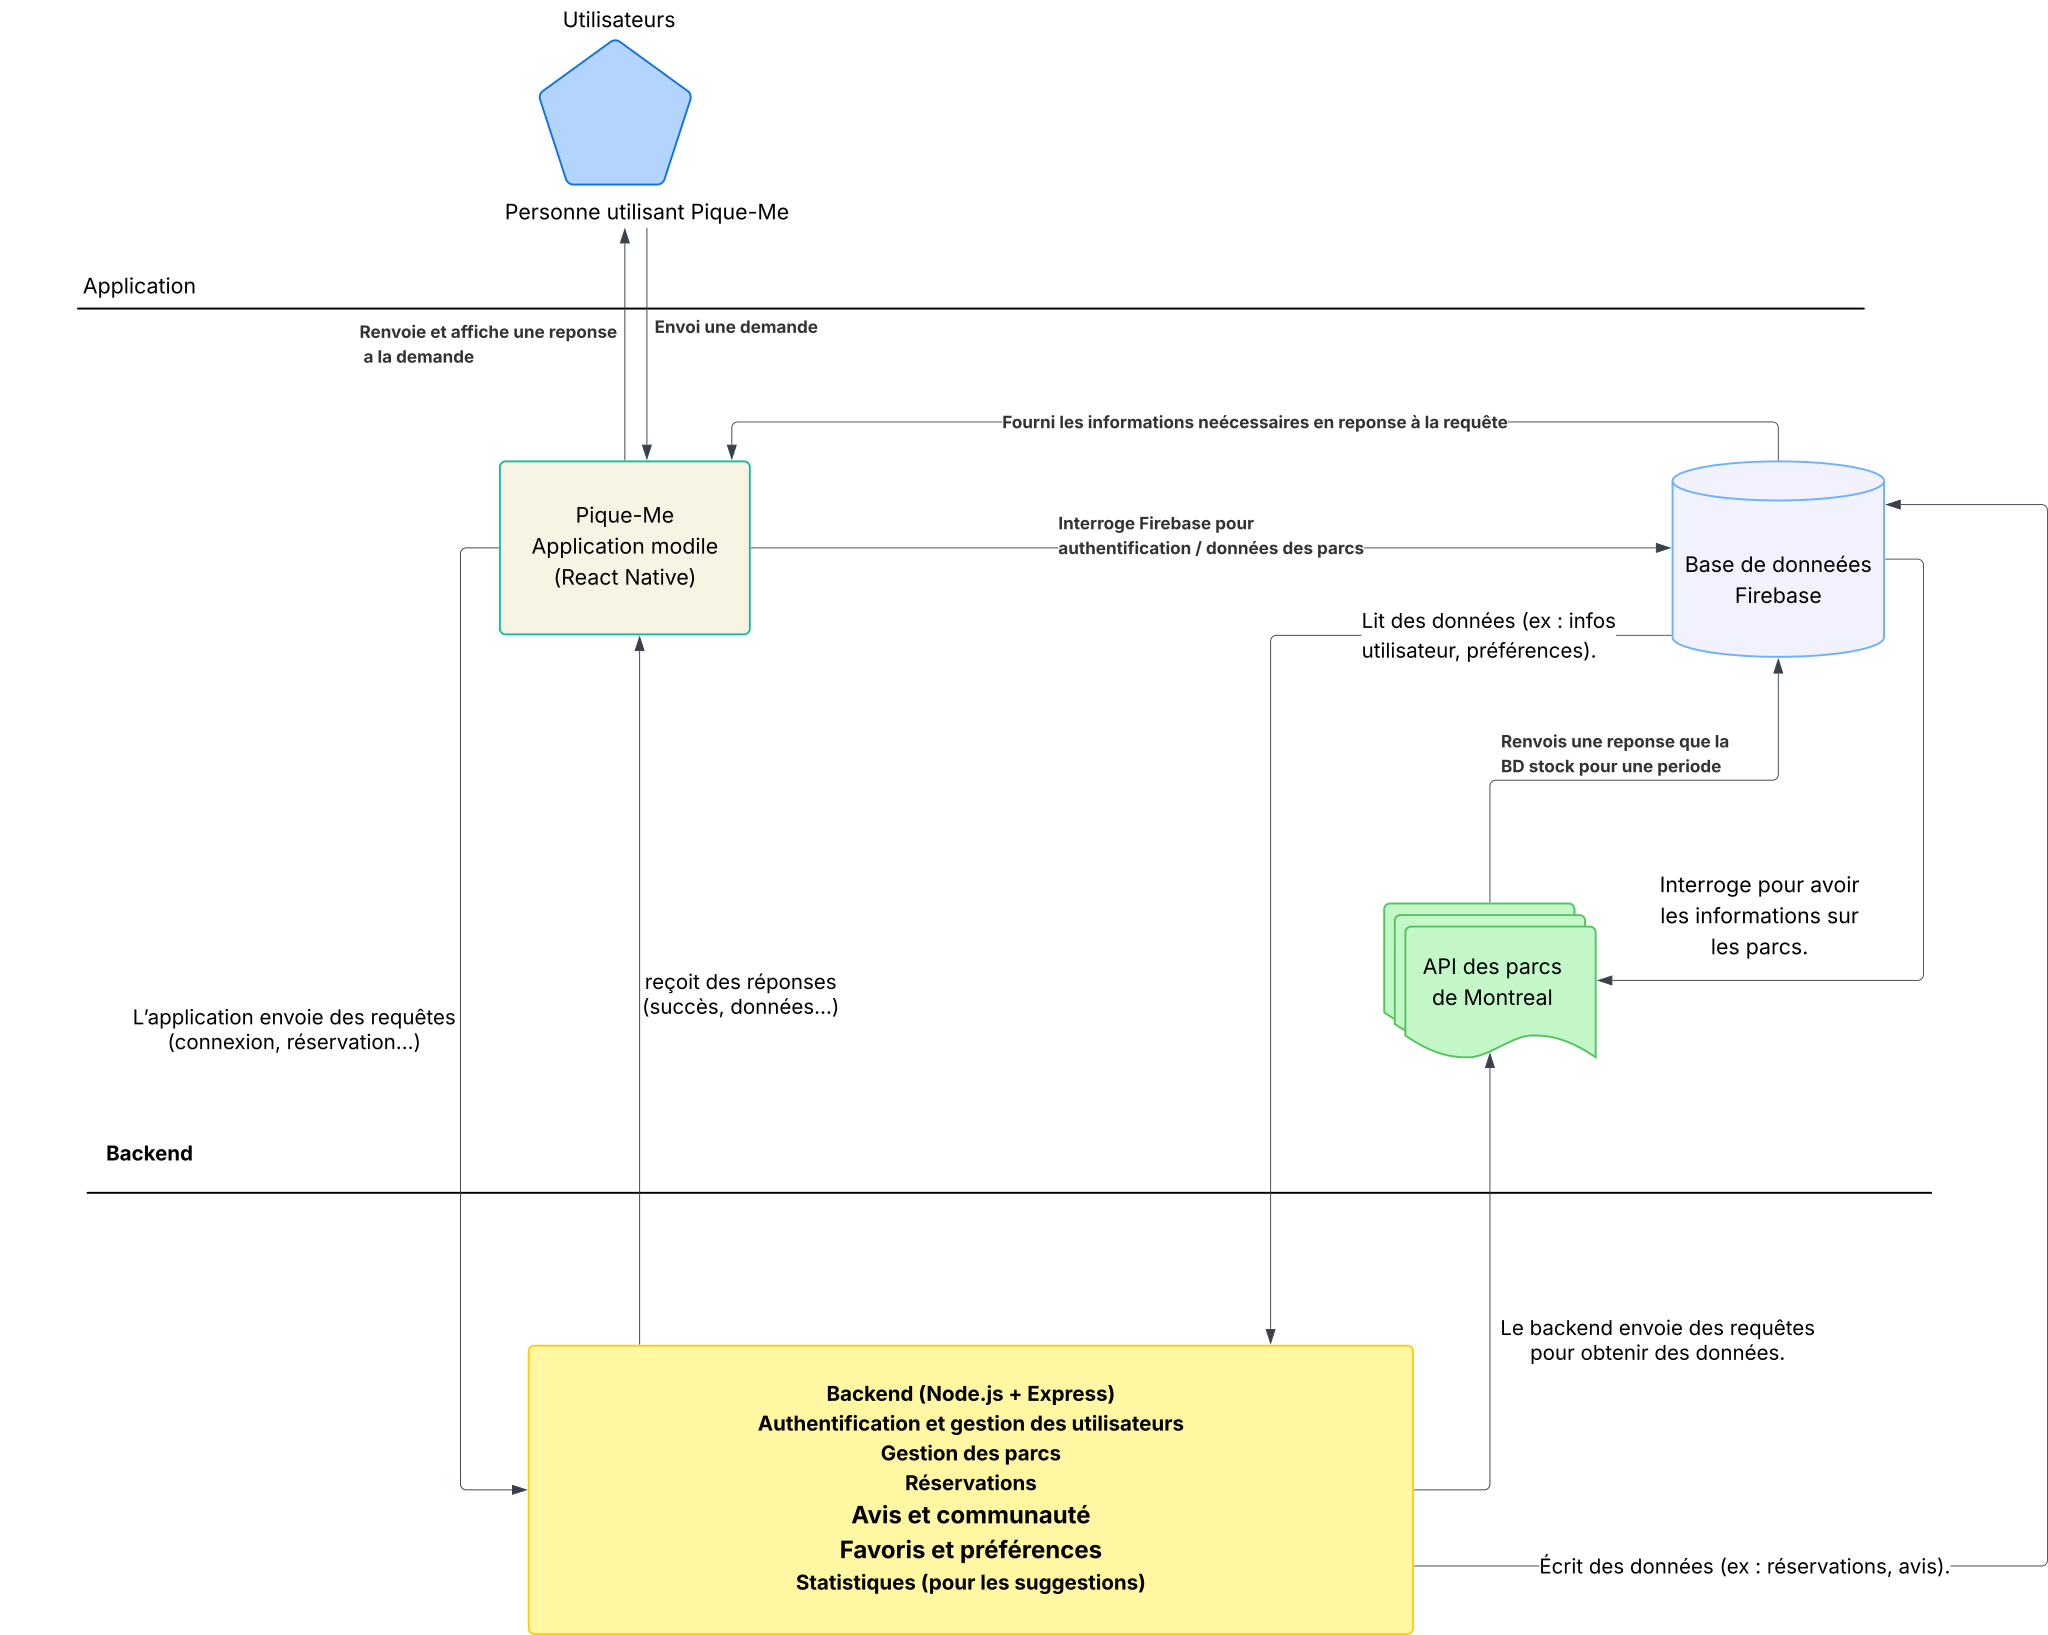
\includegraphics[width=0.9\linewidth]{attachments/architecture.pdf}
  \caption{Architecture logique de l'application Pique-Me.}
\end{figure}

\subsection{Modèle de données}

Le schéma suivant montre le modèle de données UML utilisé pour l'application Pique-Me.
Il présente les éléments importants de l'application, comme les utilisateurs, les parcs, les réservations, les événements, les équipements, les avis et les photos.
On y voit aussi comment ces éléments sont liés entre eux. 

\begin{figure}[h!]
  \centering
  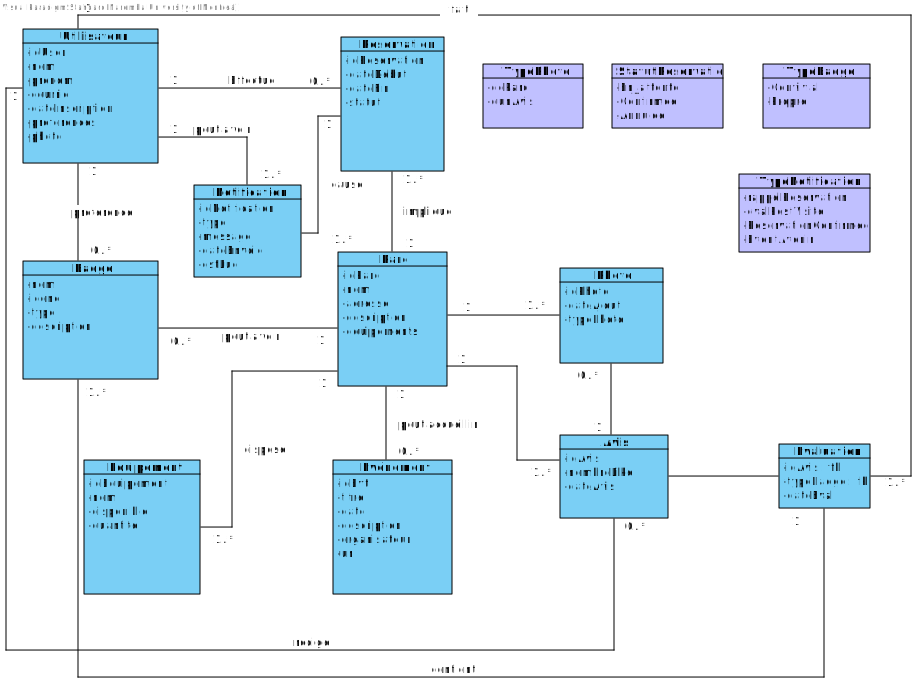
\includegraphics[width=0.9\linewidth]{attachments/donnee.pdf}
  \caption{Diagramme Entité–Association de Pique-Me.}
\end{figure}

\subsection{Choix technologiques et justifications}

\begin{itemize}
  \item \textbf{React Native + Expo :} développement multiplateforme rapide, composants UI réutilisables, configuration simplifiée.
  \item \textbf{Node.js + Express :} création d'une API REST structurée et découplée de l'interface.
  \item \textbf{Firebase :} base de données temps réel, authentification sécurisée, simplicité de déploiement.
  \item \textbf{API Ville de Montréal :} source officielle des données des parcs.
  \item \textbf{Expo Location :} géolocalisation pour rechercher les parcs à proximité.
\end{itemize}

%----------------------------------------------------------
\subsection{Diagrammes d'activités (flux utilisateurs)}
%----------------------------------------------------------

\subsubsection{Inscription et connexion}

Ce diagramme illustre les étapes principales du flux d'inscription et de connexion de l'utilisateur.

\begin{figure}[h!]
  \centering
  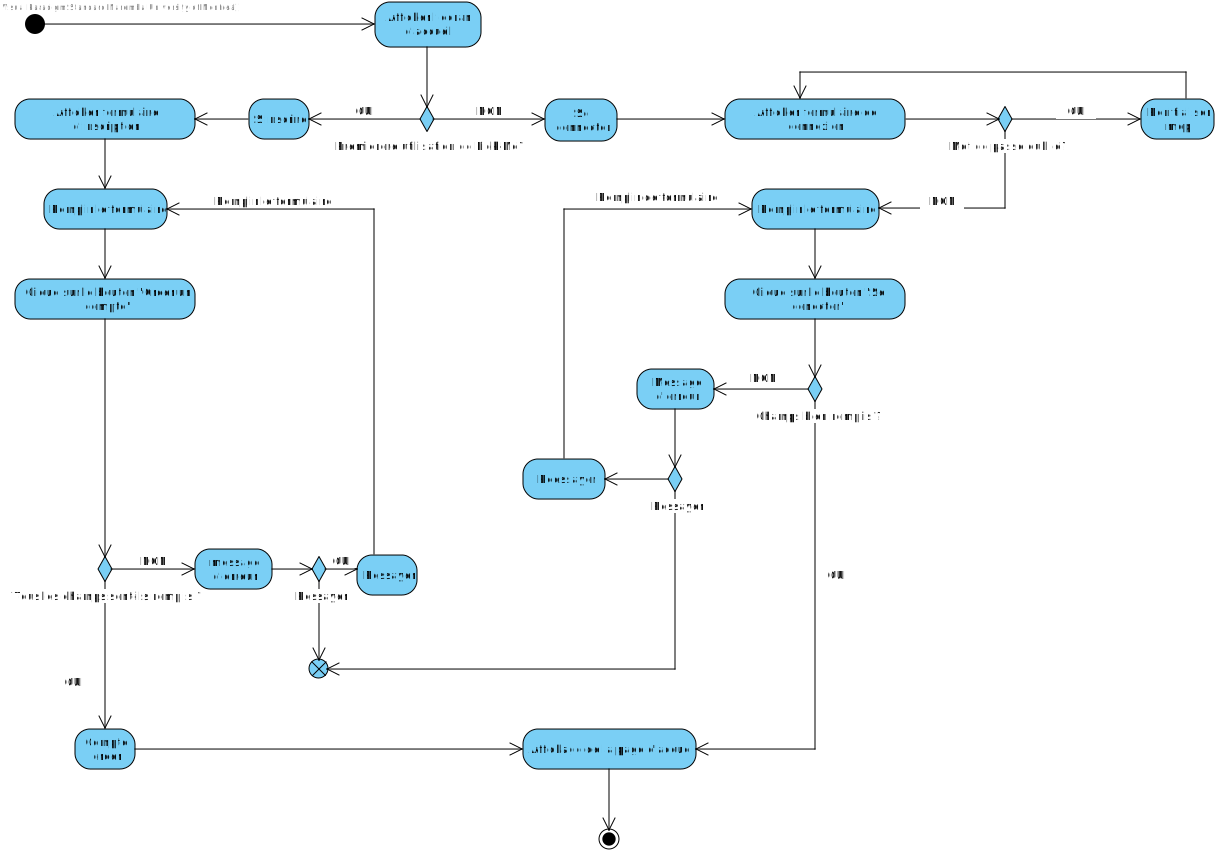
\includegraphics[width=0.9\linewidth]{attachments/Inscription_Connexion.pdf}
  \caption{Flux : Inscription et connexion}
\end{figure}

\subsubsection{Recherche et filtrage de parcs}

Ce diagramme montre le processus de recherche et de filtrage des parcs par l'utilisateur.

\begin{figure}[h!]
  \centering
  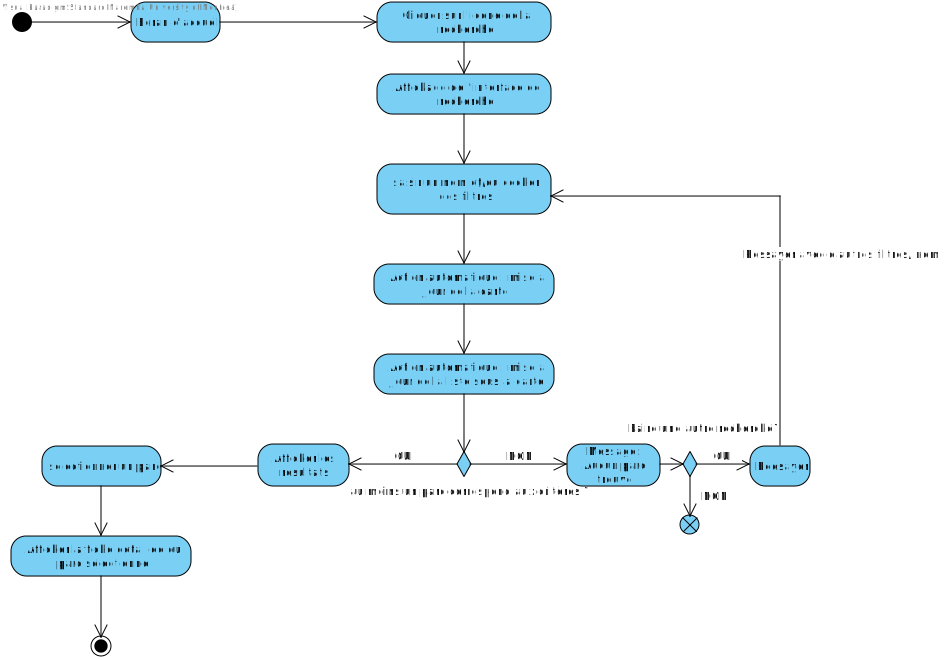
\includegraphics[width=0.9\linewidth]{attachments/Recherche_Filtrage_Parcs.pdf}
  \caption{Flux : Recherche et filtrage de parcs}
\end{figure}

\subsubsection{Réservation d'un emplacement}

Parcours utilisateur pour choisir un emplacement sur la carte du parc, sélectionner une date/heure puis confirmer la réservation.

\begin{figure}[h!]
  \centering
  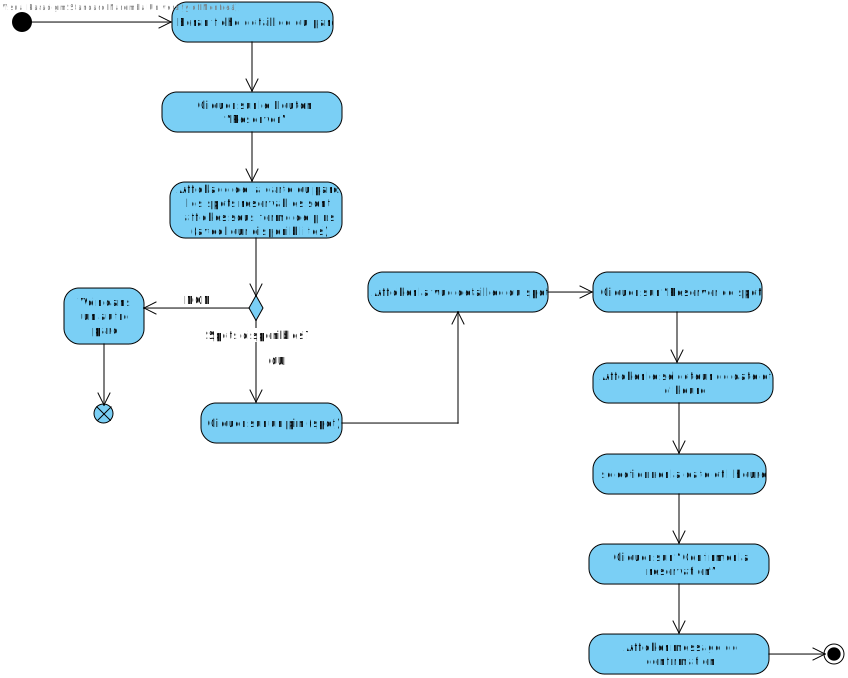
\includegraphics[width=0.9\linewidth]{attachments/Reservation_d_un_emplacement.pdf}
  \caption{Flux : Réservation d'un emplacement}
\end{figure}

\subsubsection{Réservation d'une activité}

Étapes pour sélectionner une activité dans la fiche du parc, choisir un créneau horaire et confirmer la réservation.

\begin{figure}[h!]
  \centering
  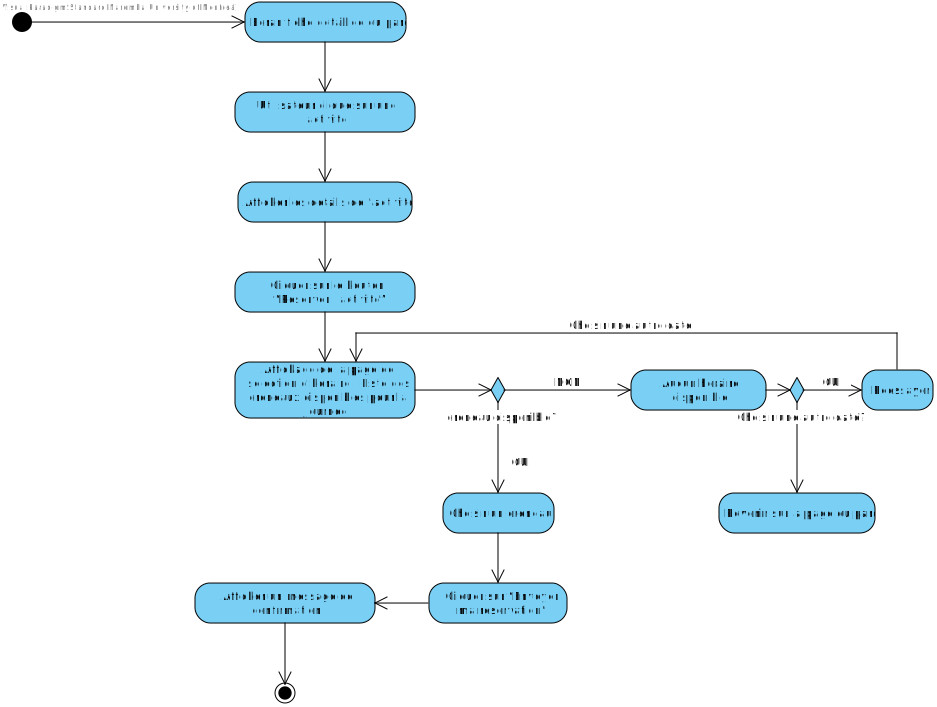
\includegraphics[width=0.9\linewidth]{attachments/Reservation_Activite.pdf}
  \caption{Flux : Réservation d'une activité}
\end{figure}

\subsubsection{Ajout ou retrait d'un favori}

Deux cas sont couverts : retirer un parc des favoris depuis la fiche du parc ou depuis la page des favoris.

\begin{figure}[h!]
  \centering
  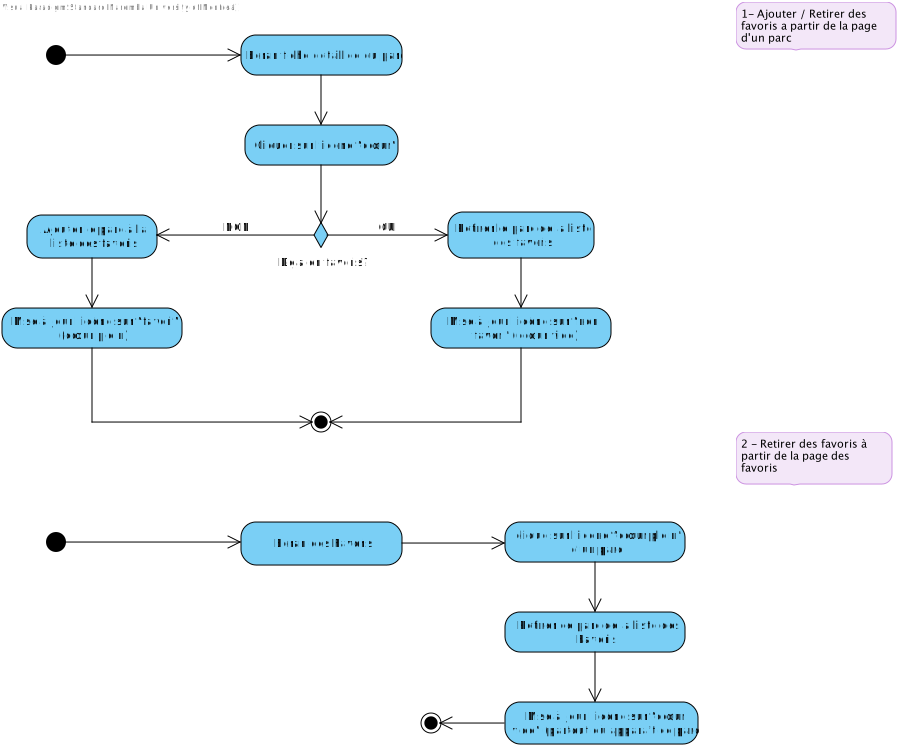
\includegraphics[width=0.9\linewidth]{attachments/Ajout_retrait_d_un_favori.pdf}
  \caption{Flux : Ajout / retrait d'un favori}
\end{figure}

\subsubsection{Ajout d'un avis}

L'utilisateur descend jusqu'à la section « Avis », saisit un commentaire, ajoute éventuellement une image, puis envoie son avis.

\begin{figure}[h!]
  \centering
  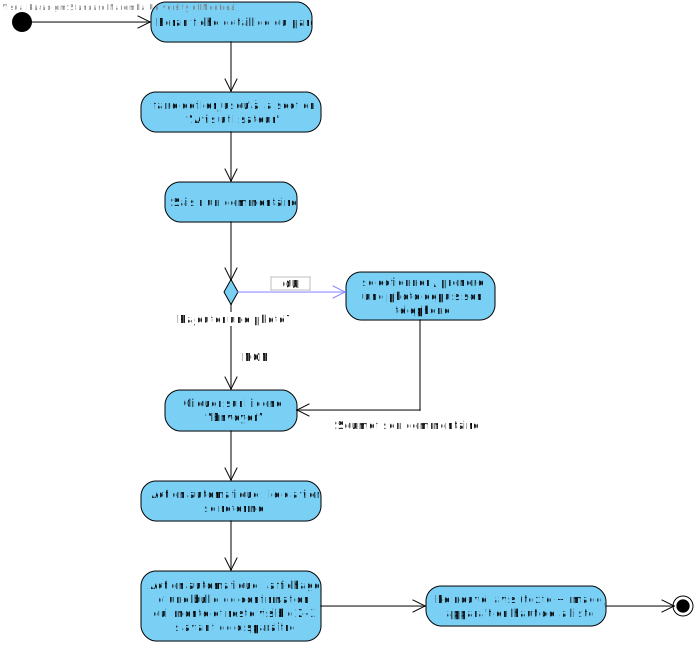
\includegraphics[width=0.9\linewidth]{attachments/Ajouter_un_avis_spot.pdf}
  \caption{Flux : Ajout d'un avis}
\end{figure}

\subsubsection{Sondage post-visite}

Après la visite, l'utilisateur reçoit une notification « Would you Pick-Me again ? », sélectionne des badges et peut laisser un commentaire.

\begin{figure}[h!]
  \centering
  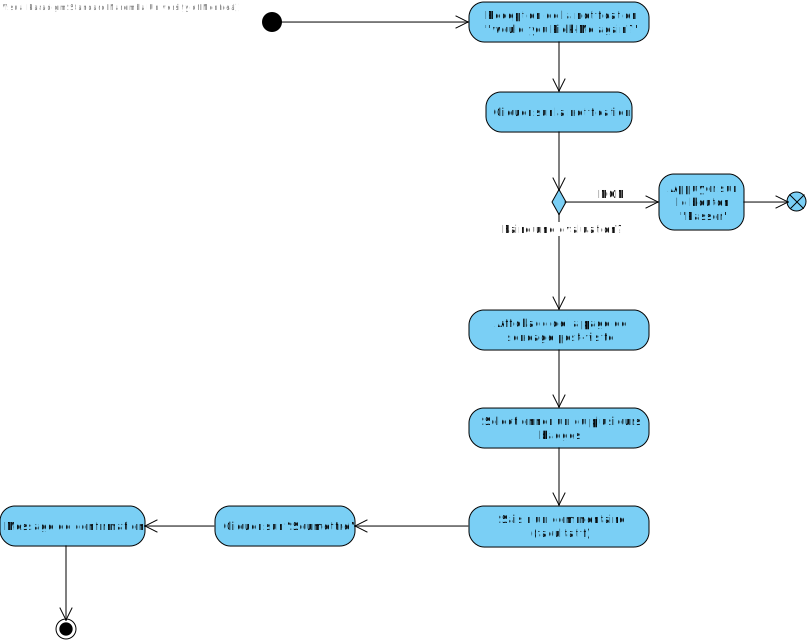
\includegraphics[width=0.9\linewidth]{attachments/Sondage_post_visite.pdf}
  \caption{Flux : Sondage post-visite}
\end{figure}

\subsection{Prototypes et maquettes}

Le design de l'application a été pensé pour offrir une expérience intuitive, visuelle et cohérente sur mobile. La maquette interactive a été conçue avec Figma.

\vspace{0.5em}
\noindent\textbf{Lien Figma :} \url{https://www.figma.com/design/kP7QEAejfvUB2yia4cleau/Pique-me?node-id=0-1}

\subsection{Contraintes et considérations}

\begin{itemize}
  \item \textbf{Techniques :} limiter le nombre d'appels vers les services externes, garantir une connexion correcte même si le réseau est lent ou instable.
  \item \textbf{Réglementaires :} respecter la vie privée des utilisateurs ; permettre la suppression de leurs données s'ils le demandent.
  \item \textbf{Fonctionnelles :} demander à l'utilisateur de confirmer sa réservation, l'annuler automatiquement s'il ne se présente pas dans l'heure, et éviter qu'un même créneau soit réservé deux fois.
\end{itemize}


% =========================================================
% 4. IMPLÉMENTATION ET RÉALISATION TECHNIQUE
% =========================================================
\section{Implémentation et réalisation technique}

Cette section présente comment nous avons transformé le projet Pique-Me en une vraie application mobile.
Après avoir défini les fonctionnalités clés, nous avons découpé l'app en petits composants simples, chacun responsable d'une tâche précise (ex. affichage d'un parc, ajout aux favoris, formulaire de réservation…).
En cours de route, nous avons ajusté la conception. Par exemple, l'API de Montréal ne répondait pas entièrement à nos besoins : nous avons donc fusionné plusieurs sources de données, puis stocké le tout dans Firebase.
Chaque page suit un flux logique clair, et les données s'actualisent en temps réel grâce aux outils fournis par Firebase.

%----------------------------------------------------------
\begin{itemize}
\item L'\textbf{interface mobile}, développée avec React Native et Expo, affiche toutes les pages de l'application. Elle gère les gestes de l'utilisateur (clics, défilement, navigation…).
\item La \textbf{base de données en ligne}, hébergée sur Firebase, contient les informations essentielles : comptes des utilisateurs, réservations d'activités ou d'emplacements, parcs favoris et avis. Elle permet aussi de recevoir les mises à jour instantanément sans avoir à rafraîchir manuellement.

\item Un \textbf{script d'importation} a été conçu pour récupérer plusieurs ensembles de données ouvertes (emplacements des parcs, installations sportives, règles d'usage). Ces fichiers sont fusionnés, nettoyés et organisés dans une base unifiée, appelée \texttt{parks}, utilisée dans toute l'application.
\end{itemize}

Cette architecture simple évite la gestion d'un serveur complexe : tout est centralisé dans Firebase, ce qui accélère le développement et garantit une bonne réactivité sur mobile.

%----------------------------------------------------------
\subsection{Particularités rencontrées}
\begin{itemize}
\item \textbf{Découverte de Firebase :} au début du projet, nous ne connaissions pas Firebase. Il a fallu apprendre à l'utiliser, notamment pour gérer les droits d'accès, les mises à jour en temps réel, l'authentification et la structure des données. Finalement, cela nous a permis de déléguer toute la logique serveur (sécurité, réservations, notifications), ce qui a simplifié considérablement notre code.
\item \textbf{Gestion correcte des favoris :} pour éviter les doublons ou les incohérences, nous avons conçu une fonction centrale qui gère l'ajout ou la suppression de favoris depuis n'importe quelle page. Ainsi, les états restent synchronisés automatiquement entre l'accueil, la page de favoris et les fiches de parc.

\item \textbf{Carte et affichage limité des parcs :} pour ne pas saturer visuellement la carte ni ralentir les performances, nous avons limité l'affichage des « pins » aux parcs situés dans un rayon de 2 km autour de l'utilisateur. Cela rend la carte plus fluide et plus lisible, surtout dans les quartiers denses.

\item \textbf{Réservations concurrentes :} pour éviter que deux utilisateurs réservent le même emplacement au même moment, la base de données vérifie chaque requête en temps réel. Si le créneau est déjà pris, un message d'erreur clair est retourné immédiatement.


\end{itemize}

%----------------------------------------------------------
\subsection{Flux principaux par page}

\paragraph{Accueil \\}
Cette page met en avant deux types de parcs : ceux recommandés selon les préférences de l'utilisateur (plein air, sport, famille, etc.), et ceux situés à proximité (sur un rayon de deux kilomètres à la ronde). Chaque carte de parc peut être cliquée pour accéder à sa fiche détaillée, ou ajoutée directement aux favoris.

\paragraph{Recherche \\}
L'utilisateur peut rechercher un parc par mot-clé ou appliquer des filtres (type de parc, activités disponibles, etc.).  
\textbf{Astuce de vitesse :} au lieu d'attendre que tous les résultats soient prêts, la page affiche immédiatement quelques parcs très pertinents. En parallèle, le reste de la liste continue à se charger discrètement. Cela donne une impression de fluidité et de réactivité.

\paragraph{Détail d'un parc \\}
Chaque fiche de parc présente une image principale, les équipements disponibles ou activités, et deux boutons :  
 « Réserver » pour choisir un créneau ;  
 une icône en forme de cœur pour ajouter ou retirer ce parc de la liste personnelle.  
L'ensemble est mis à jour en temps réel via Firebase.

\paragraph{Réservation \\}
L'utilisateur sélectionne un emplacement et un créneau horaire. Une confirmation visuelle apparaît.  
60 minutes avant l'heure choisie, une notification est envoyée. Si l'utilisateur ne se présente pas, la réservation est annulée automatiquement une heure après le début prévu.

\paragraph{Favoris \\}
Les parcs ajoutés aux favoris sont listés dans une page dédiée. Chaque carte peut être retirée en cliquant sur l'icône cœur. Toute modification est immédiatement répercutée sur les autres pages.

\paragraph{Profil \\}
Cette page permet de modifier le nom, le mot de passe et les préférences (tags). Chaque modification est enregistrée automatiquement dès que l'utilisateur quitte le champ de saisie. Les préférences servent à personnaliser les suggestions de parcs à l'accueil.

\paragraph{Avis \\}
Après une visite, l'utilisateur reçoit une notification l'invitant à donner son avis. Il peut sélectionner un ou plusieurs badges (ex. : propre, calme, familial), laisser un commentaire et ajouter une photo.  
Si un badge reçoit beaucoup de votes, le parc obtient une médaille (bronze, argent ou or), visible dans sa fiche.

%----------------------------------------------------------
\subsection{Difficultés résolues}

\begin{itemize}
  \item \textbf{Fusion de données publiques :} les informations sur les parcs étaient réparties dans plusieurs fichiers (localisation, équipements et activités). Nous avons dû croiser et nettoyer ces données pour n'avoir qu'un seul format clair à utiliser dans l'application.
  
  \item \textbf{Interrogation des API trop lente :} certaines sources prenaient jusqu'à deux minutes pour répondre. Nous avons donc décidé d'extraire leurs données à l'avance et de les importer une fois pour toutes dans Firebase.

  \item \textbf{Problèmes de réservation en double :} pour éviter que deux utilisateurs réservent le même créneau, nous avons utilisé une vérification automatique côté base de données. Si le créneau est déjà pris, un message d'erreur clair s'affiche.

  \item \textbf{Affichage pas toujours à jour :} au début, il arrivait que les favoris ou les avis ne se mettent pas à jour tout de suite. Nous avons corrigé cela en connectant directement les composants d'affichage à Firebase. Ainsi, tout changement est visible en temps réel, sans avoir besoin de recharger l'écran.
\end{itemize}

%----------------------------------------------------------



% =========================================================
% 5. ÉVALUATION
% =========================================================
\section{Évaluation}
\subsection{Tests unitaires et fonctionnels}
\subsection{Évaluation de performance}
\subsection{Évaluation d'utilisabilité}
\subsection{Comparaison avec les objectifs initiaux}

% =========================================================
% 6. DISCUSSION CRITIQUE
% =========================================================
\section{Discussion critique}

La version actuelle de \textit{Pique-Me} atteint son objectif premier :
offrir, sur mobile, un moyen simple de découvrir les parcs de Montréal,
de réserver un emplacement et de partager son expérience. 

\medskip\noindent
\textbf{Analyse critique.}  
Le choix d'un socle « Firebase » a apporté un réel confort : pas de
serveur à maintenir, sécurité intégrée, mises à jour en temps réel
gratuites. En revanche, cette dépendance impose certaines limites :
logique métier cantonnée aux règles Firestore, format de requête parfois
rigide, et difficulté à exécuter des traitements lourds côté serveur. La structure en mini-composants
React facilite grandement la maintenance ; toutefois, elle augmente
aussi le nombre de fichiers à gérer et peut alourdir la prise en main
pour un nouveau développeur.

\medskip\noindent
\textbf{Problèmes rencontrés et solutions mises en place.}
\begin{itemize}
  \item \emph{Données éparpillées :} les informations officielles
        provenaient de trois sources lentes et incomplètes. Nous avons
        donc écrit un script d'import qui fusionne et nettoie ces
        fichiers, puis les stocke dans une seule collection
        \texttt{parks}. Temps de réponse côté appli : divisé par dix.
  \item \emph{API cartographique saturée :} afficher 500 parcs à la fois
        rendait la carte illisible. Nous limitons maintenant les
        marqueurs au rayon de 2 km ; les autres parcs se chargent au
        besoin quand on dézoome.
  \item \emph{Réservations en double :} deux utilisateurs pouvaient,
        durant les premiers tests, choisir le même créneau. Désormais,
        une transaction Firestore bloque la seconde requête et renvoie
        un message explicite.
  \item \emph{Synchronisation des favoris :} il arrivait qu'un cœur
        reste allumé sur un écran mais pas sur l'autre. Tous les
        composants « carte de parc » écoutent maintenant directement
        les changements Firebase ; l'affichage est harmonisé sans
        rechargement manuel.
\end{itemize}

\medskip\noindent
\textbf{Ce qui pourrait être amélioré avec plus de temps ou de moyens.}
\begin{itemize}
  \item \emph{Suggestions communautaires :} permettre aux utilisateurs
        d'ajouter eux-mêmes de nouveaux parcs ou équipements encore non
        répertoriés, photos à l'appui.
  \item \emph{Recommandations plus fines :} analyser les avis pour
        proposer des parcs en fonction du moment de la journée, de la
        météo ou d'événements spéciaux.
  \item \emph{Plateformes supplémentaires :} décliner l'application en
        version tablette et web pour toucher un public plus large :
        familles planifiant leurs sorties depuis un salon ou écoles
        préparant des activités extérieures.
  \item \emph{Fonctions hors ligne étendues :} permettre le
        téléchargement d'un arrondissement complet afin d'utiliser la
        recherche cartographique sans réseau du tout.
  \item \emph{Interface adaptable :} proposer un mode « gaucher »
        (boutons principaux inversés) et des options d'accessibilité
        supplémentaires (taille de police, contraste renforcé).
  \item \emph{Multilingue :} offrir l'application en français et en
        anglais (et d'autres langues à terme) afin d'être inclusive
        pour les résidents et touristes.
\end{itemize}


\medskip\noindent


% =========================================================
% 7. CONCLUSION
% =========================================================
\section{Conclusion}

Le projet \textit{Pique-Me} visait à simplifier l'expérience des citoyens dans les parcs urbains : trouver le bon lieu, réserver un espace et partager un avis. En quatre mois, nous avons livré une application mobile fluide, capable d'afficher les parcs pertinents en quelques secondes et de synchroniser réservations ou favoris en temps réel. 

\medskip\noindent
\textbf{Leçons tirées.}  
Nous avons mesuré la force et les limites d'une solution entièrement basée sur Firebase : elle accélère la mise en œuvre et la synchronisation, mais impose un format de requête strict. L'approche « mini-composants » sous React Native s'est révélée payante : chaque pièce est réutilisable et testable isolément, limitant les régressions. Enfin, fusionner plusieurs jeux de données publics nous a appris qu'un nettoyage rigoureux avant importation est indispensable pour garantir une source unique et fiable.

\medskip\noindent
\textbf{Pistes d'amélioration.}  
\begin{itemize}
  \item \emph{Fonctions communautaires élargies :} permettre aux usagers de proposer de nouveaux parcs ou équipements, photos à l'appui.
  \item \emph{Recommandations personnalisées :} intégrer la météo, l'heure de la journée et les avis pour suggérer le parc idéal à chaque instant.
  \item \emph{Accessibilité renforcée :} mode gaucher, tailles de texte adaptatives, synthèse vocale pour la navigation.
  \item \emph{Version web et tablette :} offrir la même expérience sur grand écran, utile aux familles et aux écoles.
  \item \emph{Mode hors-ligne complet :} téléchargement d'un arrondissement pour une consultation sans réseau, puis synchronisation différée.
\end{itemize}

\medskip\noindent
En définitive, \textit{Pique-Me} prouve qu'une architecture simple et modulaire peut rendre un service concret et apprécié. Avec ces améliorations, nous pourrons \textbf{étendre la couverture et faire de \textit{Pique-Me} l'outil de référence des sorties dans les parcs montréalais}.



% =========================================================
% 8. REMERCIEMENTS (facultatif)
% =========================================================
\section*{Remerciements}

Nous souhaitons exprimer notre gratitude envers nos collègues \textbf{Marc Oliver Jean paul} et \textbf{Lallia Diakité}, avec qui nous avons partagé le développement de ce projet dans le cadre du cours \textit{Interface personne-machine}. Leur collaboration, leur écoute et leur motivation ont grandement contribué à la réussite de ce travail.

Nous remercions également \textbf{M. Louis-Édouard Lafontant}, notre enseignant, pour son accompagnement tout au long de la session. Présent à chaque étape, il a su répondre à toutes nos questions avec rigueur et bienveillance, parfois dans le cadre de discussions (très) longues mais toujours constructives. Il n'a pas hésité à nous faire retravailler plusieurs éléments pour atteindre un meilleur rendu.

Enfin, nous tenons à saluer \textbf{notre propre engagement} : malgré une session intense, nous avons su rester investis, rigoureux et persévérants, jusqu'à la finalisation de ce projet.


% =========================================================
% 9. RÉFÉRENCES
% =========================================================
\section*{Références}

\begin{itemize}
  \item Lafontant, L.-É. \textit{Supervision, encadrement et conseils}. 

  \item Google. (2024). \textit{Documentation Firebase}. Disponible en ligne : \url{https://firebase.google.com/docs}

  \item Ville de Montréal. (2024). \textit{API publiques — données sur les parcs, équipements et activités}. \emph{(....)}.

  \item Meta. (2024). \textit{Documentation React Native}. Composants de base, navigation et gestion d'état. \emph{(....)}.

  \item OpenAI. (2025). \textit{Assistance à la rédaction et au débogage via ChatGPT}. \url{https://chat.openai.com}
\end{itemize}


% =========================================================
% 10. ANNEXES
% =========================================================
\appendix
\section{Annexes}

\end{document}
